%!TEX root = thesis.tex

\chapter{Combining nonparametric morphologies with human and machine intelligence}
\label{chap:4}



%%----------------------------------------------------------------------------------------------------------------------------------------------------
%%   INTEGRATING MACHINE CLASSIFIERS 
%%----------------------------------------------------------------------------------------------------------------------------------------------------
\section{Efficiency through incorporation of machine classifiers} \label{sec: machine}

We construct the full Galaxy Zoo Express by incorporating supervised 
learning, the machine learning task of inference from labelled training data. 
The training data consist of a set of training examples, and must include
an input feature vector and a desired output label.  Generally speaking,
a supervised learning algorithm analyses the training data and produces a 
function that can be mapped to new examples. A properly optimized algorithm will 
correctly determine class labels for unseen data. By processing human classifications 
through SWAP, we obtain a set of binary labels by which we can train a machine 
classifier. We briefly outline the technical details of our machine below,  turning
towards the decision engine we develop in Section~\ref{sec: decision engine}. 



%%----------------------------------------------------------------------------------------------------------------------------------------------------
%%   RANDOM FORESTS
%%----------------------------------------------------------------------------------------------------------------------------------------------------
\subsection{Random Forests}
We use a Random Forest (RF) algorithm~\citep{Breiman2001},  
an ensemble classifier that operates by
 bootstrapping the training data and constructing a multitude of individual decision 
tree algorithms, one for each subsample.  
An individual decision tree works by deciding which of 
the input features best separates the classes. It does this by performing 
splits on the values of the input feature that minimize the classification 
error. These feature splits proceed recursively. Decision trees alone are
 prone to over-fitting, precluding them from generalizing 
well to new data. Random Forests mitigate this effect by combining the 
output labels from a multitude of decision trees.  Specifically, we use the 
\texttt{RandomForestClassifier} from the Python module \texttt{scikit-learn}
\citep{scikit-learn}. 


%%----------------------------------------------------------------------------------------------------------------------------------------------------
%%   CROSS-VALIDATION
%%----------------------------------------------------------------------------------------------------------------------------------------------------
\subsection{Grid Search and Cross-validation}
Of fundamental importance is the task of choosing an algorithm's hyperparameters, 
values which determine how the machine learns.   For a RF, key quantities include
 the maximum depth of individual trees (\texttt{max\_depth}), the number of trees
in the forest (\texttt{n\_estimators}), and the number of features to consider when 
looking for the best split (\texttt{max\_features}). 
The goal is to determine which values will optimize 
the machine's performance and thus these values cannot be chosen \textit{a priori}. 
We perform a grid search with $k$-fold cross-validation whereby the 
training sample is split into $k$ subsamples. One subsample is withheld to 
estimate the machine's performance while the remaining data are used to train the machine. 
This is performed $k$ times and the average performance
value is recorded. The entire process is repeated for every combination of the 
 hyperparameters in the grid space and values that optimize the output are chosen. 
In this work we let $k=10$, however, we leave this as an adjustable input parameter.
In the interest of computational speed, we set \texttt{n\_estimators} $=30$ and 
perform the grid search for \texttt{max\_depth} over the range $[5,16]$, and 
\texttt{max\_features} over the range $[\sqrt{D}, D]$,
where $D$ is the number of features in the feature vector, described below.
 

%%----------------------------------------------------------------------------------------------------------------------------------------------------
%%   FEATURE REPRESENTATION AND PRE-PROCESSING
%%----------------------------------------------------------------------------------------------------------------------------------------------------
\subsection{Feature Representation and Pre-Processing}
The feature vector on which the machine learns is composed of $D$ individual 
numeric quantities associated with the subject that the machine uses to discern 
that subject from others in the training sample. 
To segregate~\feat~from~\notfeat, we draw on ZEST \citep{Scarlata2007} and compute
 concentration, asymmetry, Gini coefficient, and M$_{20}$, 
the second-order moment of light for the brightest 20\% of galaxy pixels as
measured from SDSS DR12 $i$-band imaging (see Appendix \ref{sec: measuring morphology}). 
Coupled with SExtractor's measurement of ellipticity \citep{sextractor}, 
we provide the machine with a $D=5$ dimensional morphology parameter space.
These non-parametric diagnostics have long been used to distinguish between early- and late-type galaxies 
in an automated fashion \cite[e.g.,][]{Abraham1996, Bershady2000, Conselice2000, Abraham2003, Conselice2003, Lotz2004, Snyder2015}.
Because the RF algorithm handles a variety of input formats, the only pre-processing 
step we perform is the removal of poorly-measured morphological indicators, i.e. catastrophic failures.



%%%-------------------------------------------------------
%%%  FIGURE:   LEARNING CURVE
%%%-------------------------------------------------------
\begin{figure}[t!]
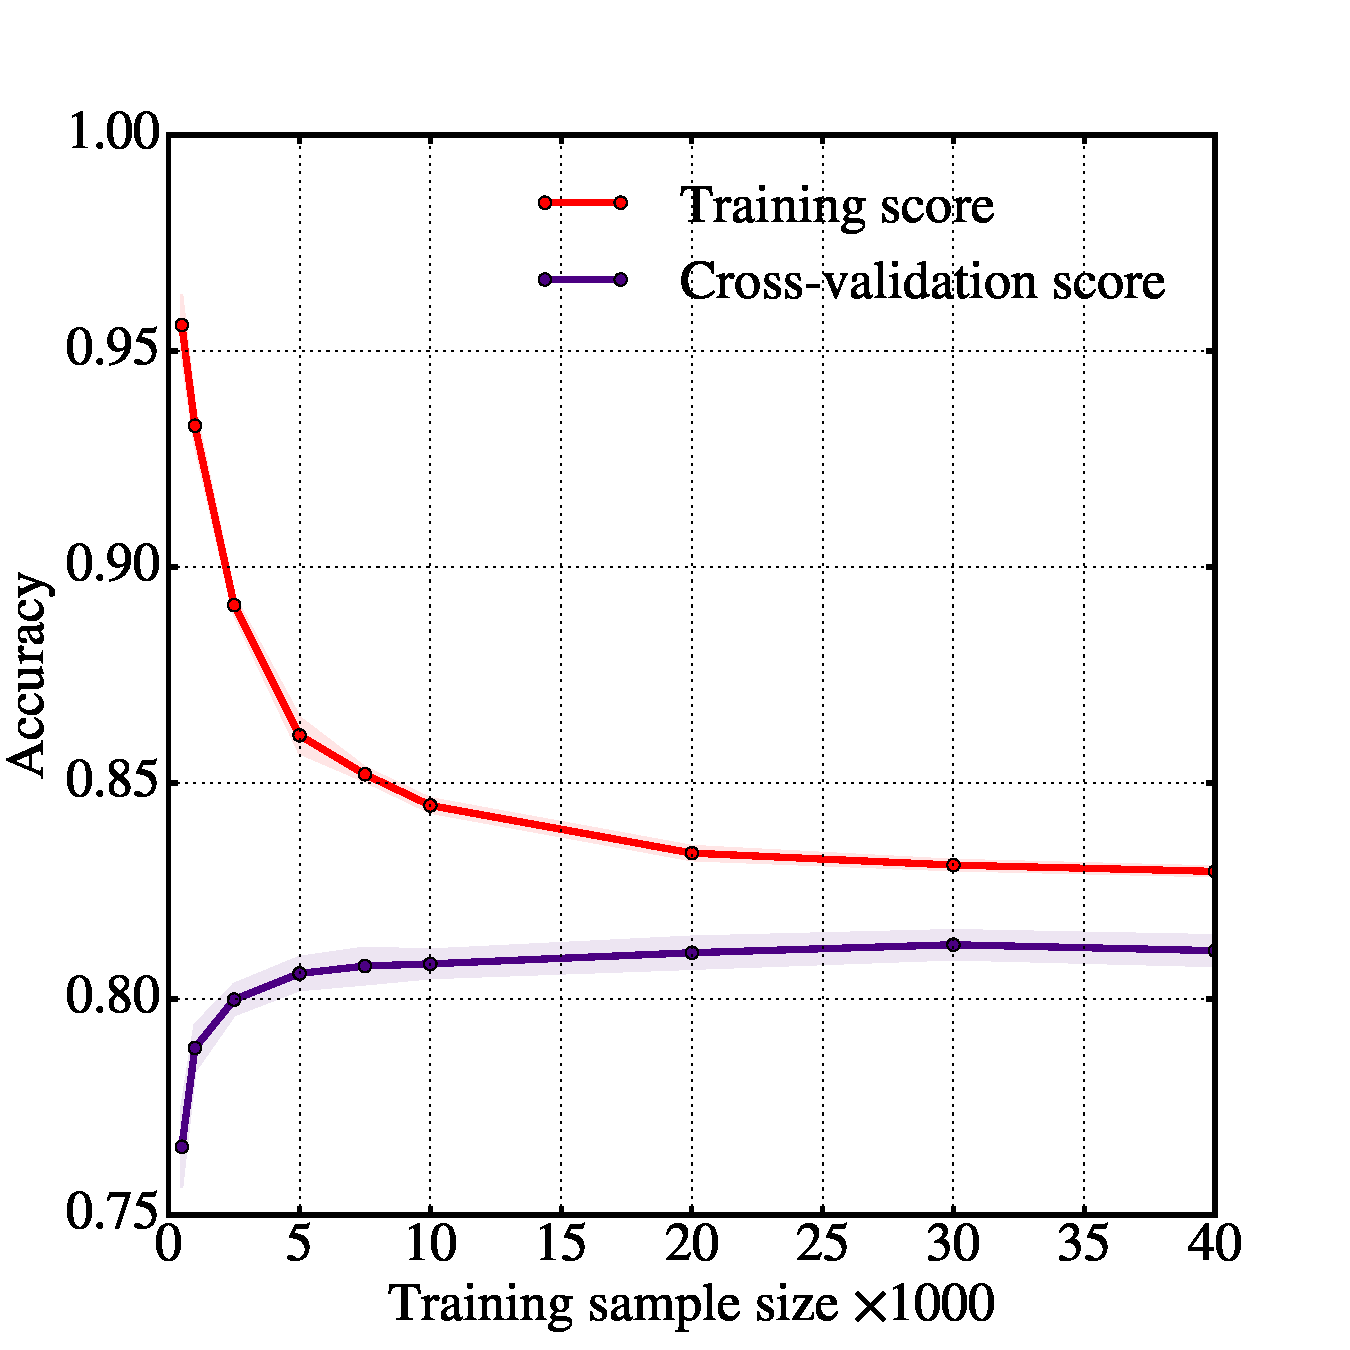
\includegraphics[width=3.25in]{Figures/human_machine/f6.pdf}
\caption[Random Forest learning curve]{Learning curve for a Random Forest with fixed hyperparameters. These curves show the mean accuracy computed during cross-validation and on the training sample, where the shaded regions denote the standard deviation. When the training sample size is small, the machine accurately identifies its own training sample but is unable to generalize to unseen data as evidenced by a low cross-validation score. As the training sample size increases, the cross-validation score increases. This behaviour plateaus indicating that larger training samples provide little in additional performance. \label{fig: learning curve}}
\end{figure}


%%----------------------------------------------------------------------------------------------------------------------------------------------------
%%   DECISION ENGINE 
%%----------------------------------------------------------------------------------------------------------------------------------------------------
\subsection{Decision Engine}\label{sec: decision engine}
A number of decisions must be addressed before attempting to train the machine. 
In particular, which subjects should be designated as the training sample? 
When should the machine attempt its first training session? 
When has the machine's performance been optimized such that it will successfully
generalize to unseen subjects? The field of machine learning provides few hard rules 
for answering these questions, only guidelines and best practices. 
Here we briefly discuss our approach for the development of our decision engine.

%%%-------------------------------------------------------
%%%  FIGURE:    FULL GZX PERFORMANCE
%%%-------------------------------------------------------
\begin{figure*}[t!]
\centering
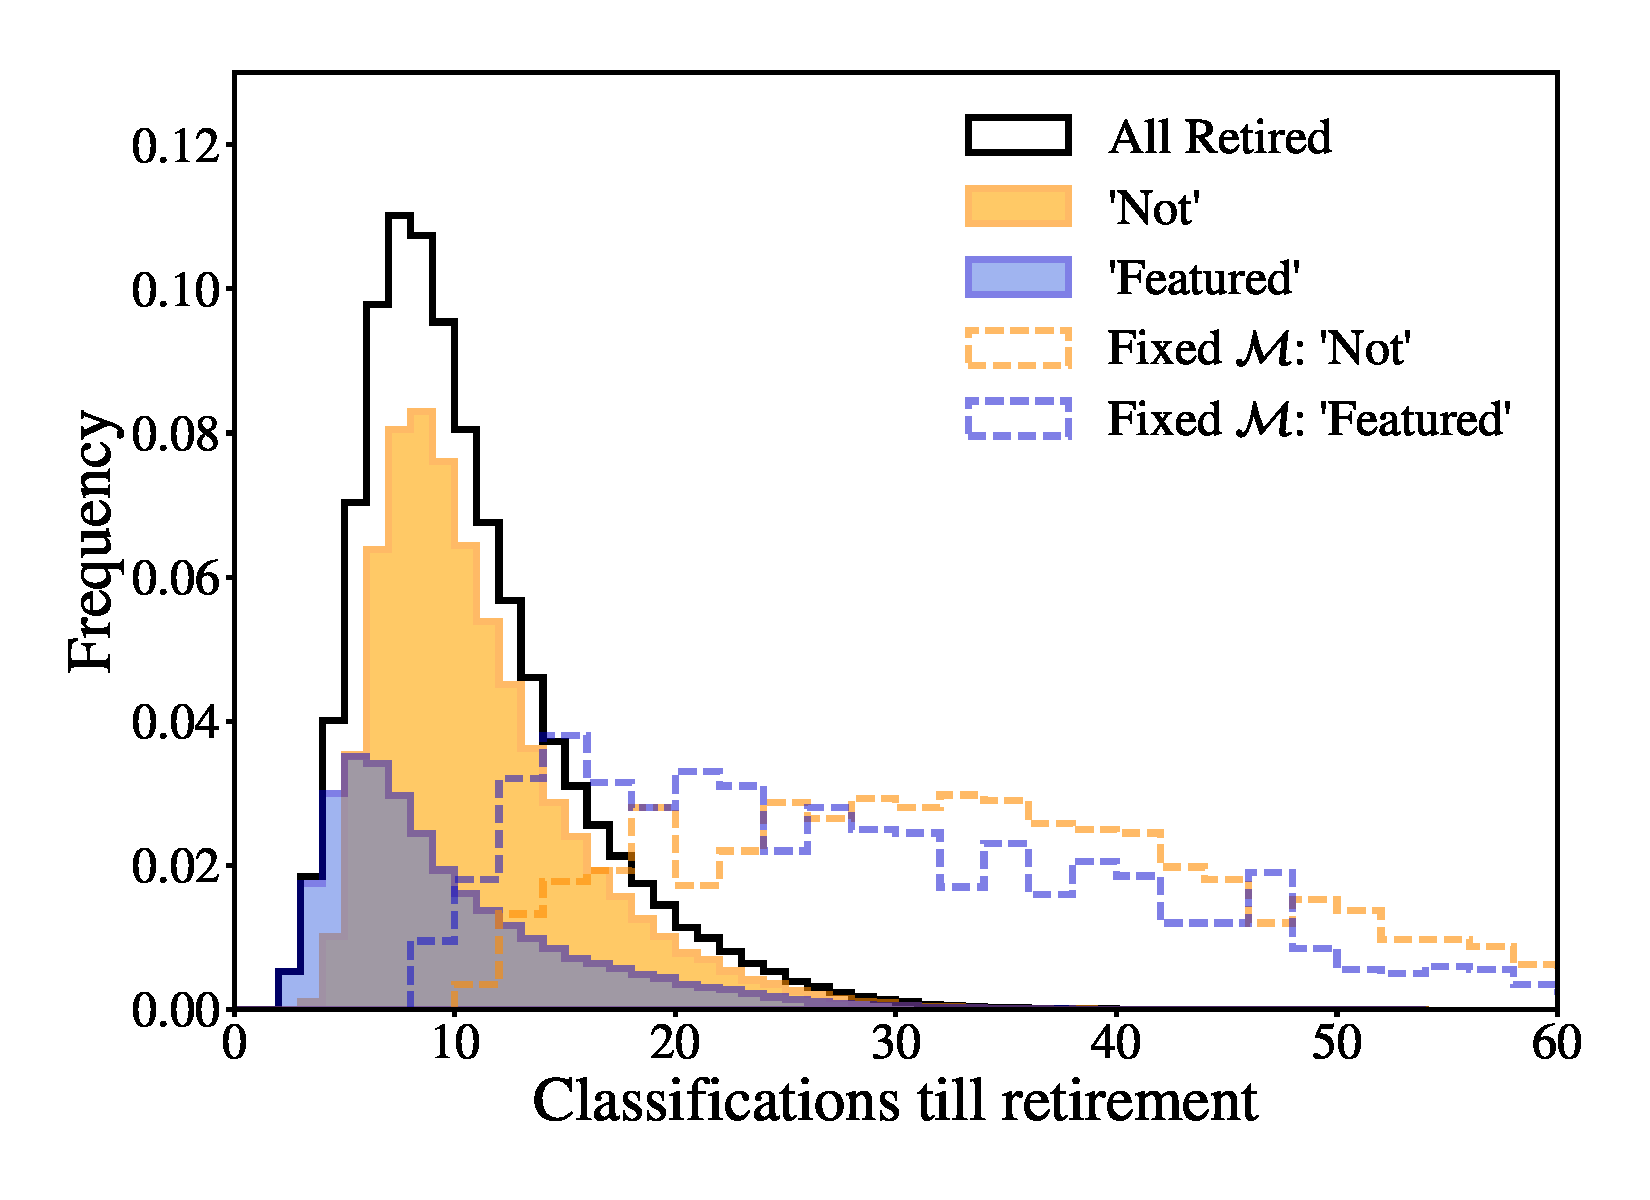
\includegraphics[width=5.5in]{Figures/human_machine/f7.pdf}
\caption[Performance of the human+machine combination -- Galaxy Zoo: Express]{By incorporating a machine classifier, GZX (red) increases the classification rate by an order of magnitude compared to GZ2 (dashed dark blue) and out-performs the SWAP-only run (light blue), retiring more than 200K subjects in just 27 days of GZ2 project time. The dashed black line marks the first night the machine trains. After several additional nights of training, it is deemed optimized and allowed to retire subjects. Both humans and machine then contribute to retirement. We end the simulation after 32 days having retired over 210K galaxies. See Table~\ref{tab: summary} for details. \label{fig: money}}
\end{figure*}


As discussed in detail in Section~\ref{sec: SWAP}, SWAP yields a probability that 
a subject exhibits the feature of interest. While some machine algorithms can 
accept continuous input labels, the RF requires distinct classes. We thus use only 
those subjects which have crossed either of the retirement thresholds. 
Though we find that SWAP consistently retires 35-40\%~\feat~subjects on 
any given day of the simulation, a balanced ratio of~\feat~to~\notfeat~isn't guaranteed.
 Highly unbalanced training samples should be resampled to correct the imbalance; 
however, as we exhibit only a mild lopsidedness, we allow the machine to train on all 
SWAP-retired subjects.  

SWAP retires a few hundred subjects during the first days of the simulation.
In principle,  a machine can be trained with such a small sample, but will be unable
to generalize to unseen data. We estimate a minimum number of training samples
and the machine's ability to generalize by considering a learning curve, an illustration
of a machine's performance with increasing sample size for fixed hyperparameters. 
Figure~\ref{fig: learning curve} demonstrates such a curve wherein we plot
the accuracy from both the 10-fold cross-validation, and the trained machine
applied to its own training sample for a random sample of GZ2 subjects
required to be balanced between~\feat~and~\notfeat.  
We fix the RF's hyperparameters as follows: \texttt{max\_depth} $=8$, 
\texttt{n\_estimators } $=30$, and \texttt{max\_features} $=2$. 
When the sample size is small, the cross-validation score is low and the training 
score is high, a clear sign of over-fitting.  However, as the training 
sample size increases, the cross-validation score increases and eventually plateaus,
 indicating that larger training sets will yield little additional gain. 

We estimate this plateau begins when the training 
sample reaches 10,000 subjects and require SWAP retire at least this many 
 before the machine attempts its first training.  We estimate the machine 
has trained sufficiently if the cross-validation score fluctuates by less than 1\% 
for three consecutive nights of training to ensure we have reached the plateau.  
This requires that we record the machine's training performance each night, 
including how well it scores on the training sample, the 
cross-validation score, and the best hyperparameters. 



%%----------------------------------------------------------------------------------------------------------------------------------------------------
%%   MACHINE SHOP 
%%----------------------------------------------------------------------------------------------------------------------------------------------------
\subsection{The Machine Shop}\label{sec: machine shop}
We can now describe a full GZX simulation, which begins with human classifications 
processed through SWAP for several days.   
Once at least 10K subjects have been retired, their feature vectors are passed to 
the machine for its inaugural training. 
A suite of performance metrics are recorded by a machine agent, similar
in construction to SWAP's agents. This agent determines 
when the machine has trained sufficiently by assessing the variation
in performance metrics for all previous nights of training. 
Once the machine has been optimized, the agent introduces it to the test sample
consisting of any subject that has not yet reached retirement through SWAP 
and is not part of the gold standard sample.  

Analogous to SWAP, we generate a retirement rule for machine-classified subjects. 
In addition to the class prediction, the RF algorithm computes the probability for
each subject to belong to each class.  This probability is simply the average of
 the probabilities of each individual decision tree, where the probability of a 
single tree is determined as the fraction of subjects of class X on a leaf node.  
Only subjects that receive a class prediction of \feat with 
$p_{\mathrm{machine}} \ge 0.9$ ($p_{\mathrm{machine}} \le 0.1$ for \notfeat)
are considered retired. 
The remaining subjects have the possibility of being classified by humans 
or the machine on a future night of the simulation. 
This constitutes the core of our passive feedback mechanism. Subjects that are
not retired by the machine can instead be retired by humans, thus providing 
the machine a more fully sampled morphology parameter space on future 
training sessions. 




%%----------------------------------------------------------------------------------------------------------------------------------------------
%%   RESULTS 
%%----------------------------------------------------------------------------------------------------------------------------------------------
\section{Results} \label{sec: results}
We perform a full GZX simulation incorporating our RF with the fiducial 
SWAP run discussed in Section~\ref{sec: fiducial}. 
The machine attempts its first training on Day 8 with an initial training
sample of $\sim$20K subjects. It undergoes several additional nights 
of training, each time with a larger training sample. 
By Day 12, SWAP has provided over 40K subjects for training and the machine's 
agent has deemed the machine optimized. 
The machine predicts class labels for the remaining 230K GZ2 subjects. 
Of those, the machine retires over 70K, dramatically increasing the 
subset of retired subjects. 
We end the simulation after 32 days, having retired $\sim$210K subjects
as detailed in Table~\ref{tab: summary}. 

We present these results in Figure~\ref{fig: money} where subject retirement 
with GZX (red) is compared to our fiducial SWAP-only run (light blue) and GZ2 (dashed dark blue). 
Using the~\raw~labels as before, we compute our usual quality metrics on the 
full sample of GZX-retired subjects; reported in Table~\ref{tab: summary}. 
Accuracy and purity remain within a few percent of the SWAP-only run at 93.5\% 
and 84.2\% respectively. Instead we see a 5\% decline in the completeness. 
While the SWAP-only run identified 99\% of~\feat~subjects, incorporation
of the machine seems to miss a significant portion thus dropping GZX completeness to 94.3\%. 
We discuss this behaviour below.

By dynamically generating a training sample through a more sophisticated analysis of 
human classifications coupled with a machine classifier, we retire more than 200K 
GZ2 subjects in just 27 days.  Visual classification through SWAP alone retires as 
many in 50 days, while GZ2 requires a full year.  
Though our analysis considers only the top-level task of GZ2's decision tree, GZX suggests a tantalizing potential to increase the classification rate by an order of magnitude over the traditional crowd-sourced approach.
We next explore the composition of those classifications.



%%----------------------------------------------------------------------------------------------------------------------------------------------
%%   WHO RETIRES WHAT, WHEN? 
%%----------------------------------------------------------------------------------------------------------------------------------------------
\subsection{Who retires what, when?}  

In the top panel of Figure~\ref{fig: gzx components} we explore the individual 
contributions to GZX subject retirement from the RF (dash-dotted teal) 
and SWAP (dashed orange). The solid black line shows the total GZX retirement (SWAP+RF), while the dotted grey line depicts the fiducial SWAP-only run from 
Section~\ref{sec: fiducial} for reference. 
Two things are immediately obvious. First, each component shoulders approximately
half of the retirement burden with the machine and SWAP responsible for 
$\sim$$100$K and $\sim$$110$K subjects respectively.  
Secondly, the rate of retirement exhibited by the two components is in stark contrast.
SWAP retires at a relatively constant rate while the machine retires 
dramatically at the beginning of its application, quickly surpassing the human 
contribution, and plateaus thereafter. 
We thus clearly see three epochs of subject retirement.
In the first phase, humans are the only contributors to subject retirement.  
Once the machine is optimized, it immediately contributes more to retirement than humans.
However, the machine's performance plateaus quickly;  the third 
phase is again dominated by human classifications.

%%%-------------------------------------------------------
%%%  FIGURE:    GZX COMPONENT CONTRIBUTIONS
%%%-------------------------------------------------------
\begin{figure}[t!]
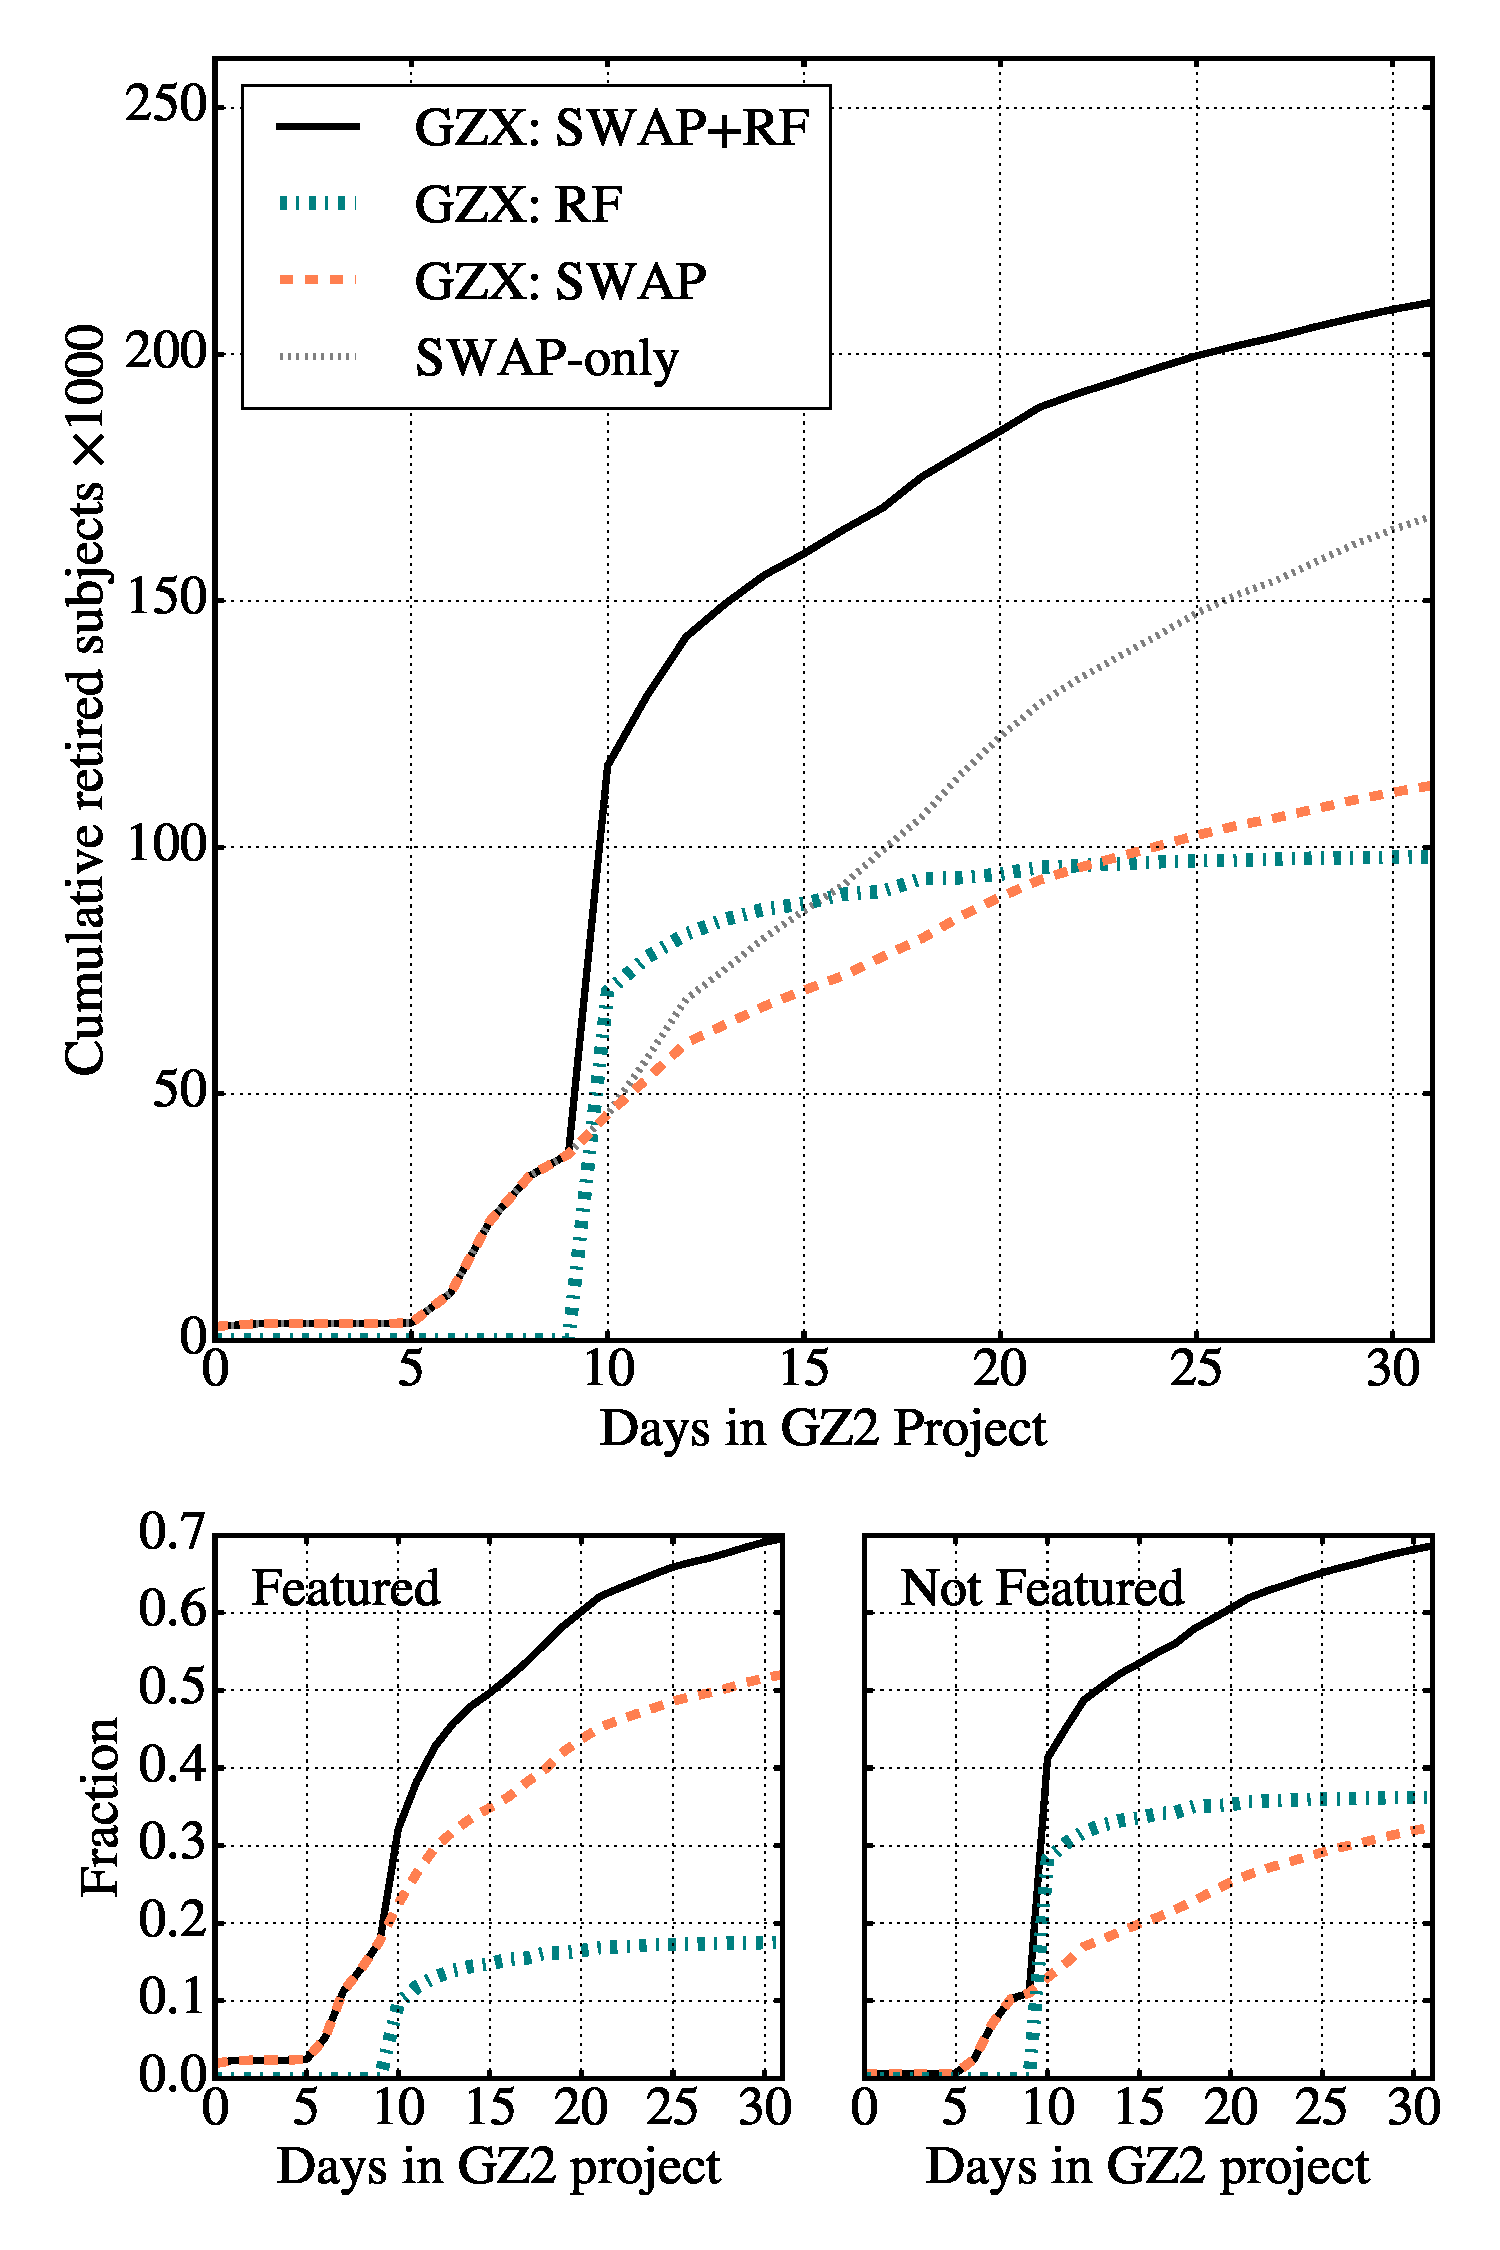
\includegraphics[width=3.5in]{Figures/human_machine/f8.pdf}
\caption[Individual contributions of human and machine to galaxy classification]{Contributions to subject retirement by both classifying agents of GZX: human (SWAP) and machine. The top panel shows cumulative subject retirement for GZX as a whole (solid black), along with that attributed to the RF (dash-dotted teal), and SWAP (dashed orange). The dotted grey line shows the fiducial SWAP-only run for comparison. Retirement totals for humans and machine are nearly equal over the course of the simulation but display different behaviours: SWAP's retirement rate is almost constant while the RF contributes substantially after its initial application and then plateaus.  The bottom panels show what fraction of GZ2 subjects are retired, separated by class label. Overall, GZX retires 73.6\% of the entire GZ2 sample in 32 days, retiring the same proportion of~\feat~and~\notfeat~subjects as indicated by the black lines. However, humans retire 30\% more~\feat~subjects than the machine, while both components retire a similar proportion of~\notfeat~subjects. \label{fig: gzx components}}
\end{figure}


\begin{table*}[]
	\centering
	\caption[Simulation summary]{Summary of key quantities for GZ2 and our various simulations. All quality metrics are calculated using~\raw~labels.}
	\label{tab: summary}
	\let\mc\multicolumn
	\begin{tabular}{lcccccc}
		
		\mc7c{ \textbf{Simulation Summary} } \\
		\hline \hline
			& Days	& Subjects Retired & Human Effort 	&  Accuracy 	& Purity 	& Completeness\\
		\mc2c{} 		& 	 	& (classifications) 	&  (\%)	    	& (\%)	& (\%)	\\
		\hline
			
		Galaxy Zoo 2	&	430 	& 285962  	& 16,340,298 	& --   	& --    	 & --   \\
		SWAP only	&	92    	& 226124          & 2,298,772	& 95.7 	& 86.7	 & 99.0     \\
		SWAP+RF   	& 32  	& 210543 	& 932,017 	& 93.5    	& 84.2    	& 94.3      \\
		\hline
	\end{tabular}
\end{table*}
%%%-------------------------------------------------------
%%%  FIGURE:    MACHINE GETS IT RIGHT!!!
%%%-------------------------------------------------------
\begin{figure*}[t!]
\centering
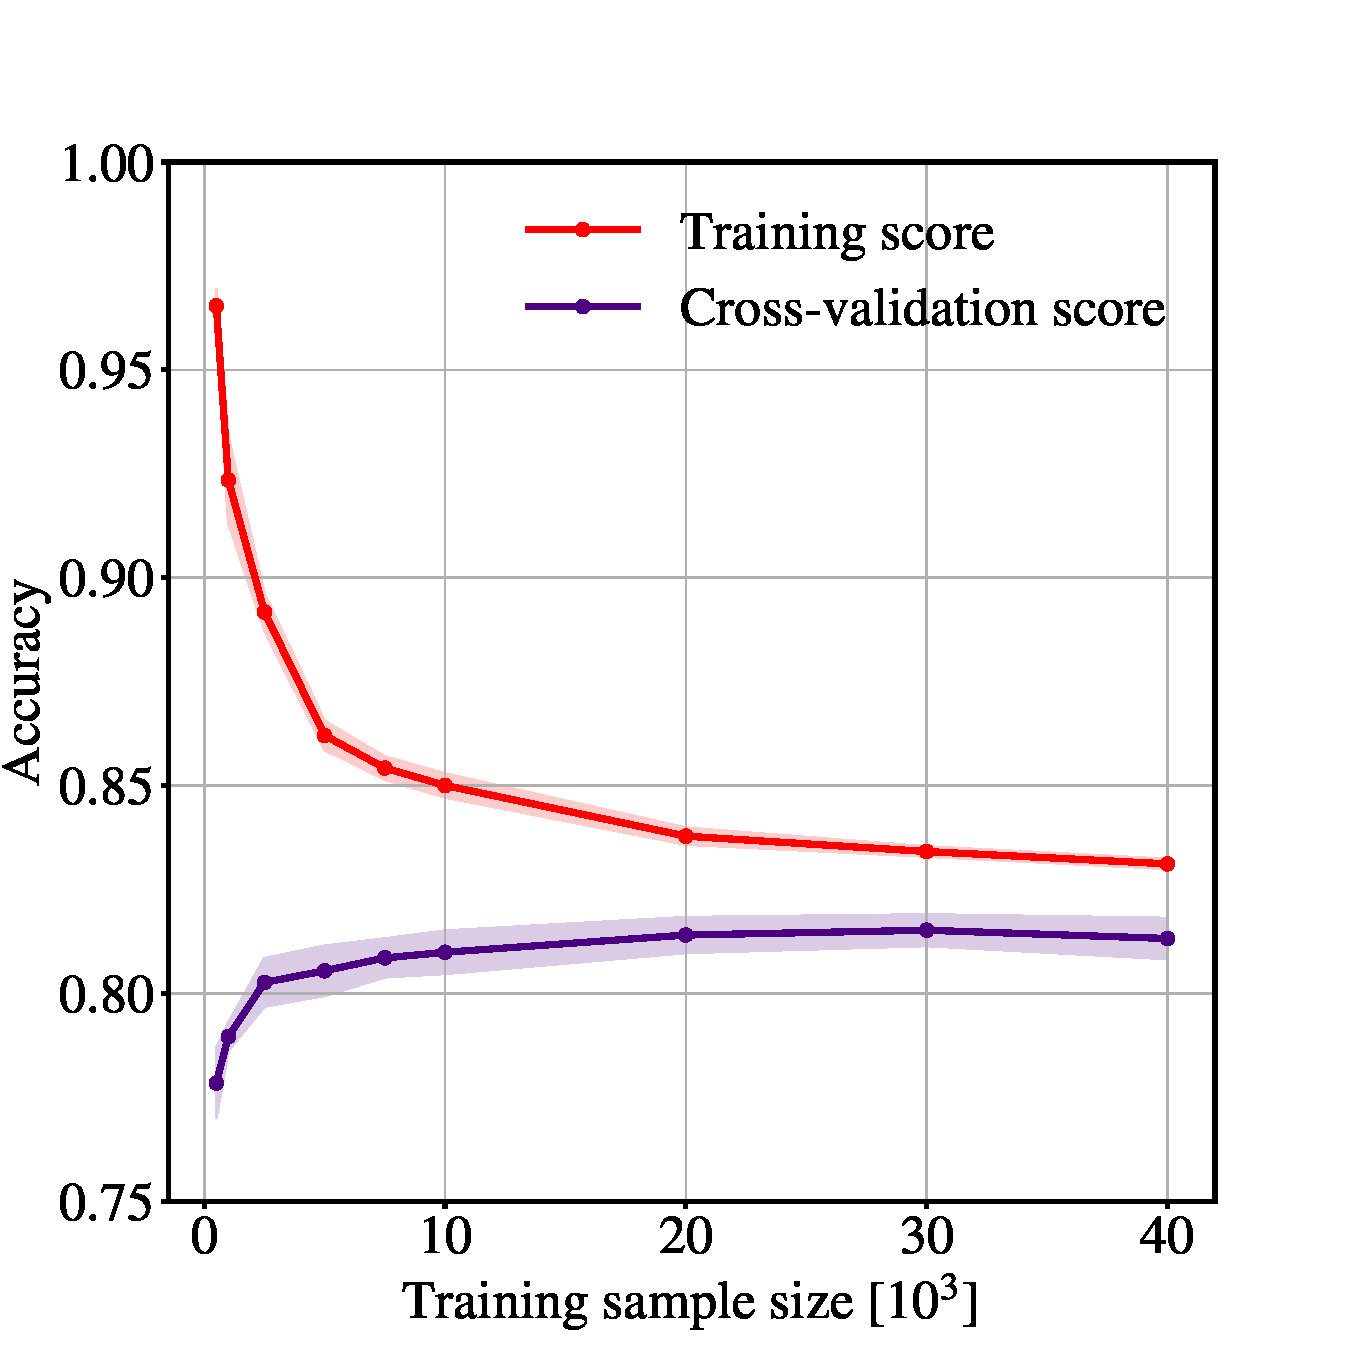
\includegraphics[width=6.5in]{Figures/human_machine/f9.pdf}
\caption[Random subsample of galaxy jpegs identified as false positives by the Random Forest]{A random subsample of subjects identified as false positives: labelled by machine as~\feat, but as~\notfeat~according to~\raw. We display \fsmooth~in the lower left corner, that is, the fraction of volunteers who classified the subject as `smooth' (\notfeat). Values are typically between 0.5 and 0.65 indicating that GZ2 volunteers did not reach a strong consensus. Fortunately, the machine is able to identify these subjects as~\feat~due to their measured morphology diagnostics. \label{fig: machine false pos}}
\end{figure*}


%%%-------------------------------------------------------
%%%  FIGURE:   CAS DISTRIBUTIONS 
%%%-------------------------------------------------------
\begin{figure*}[t!]
\centering
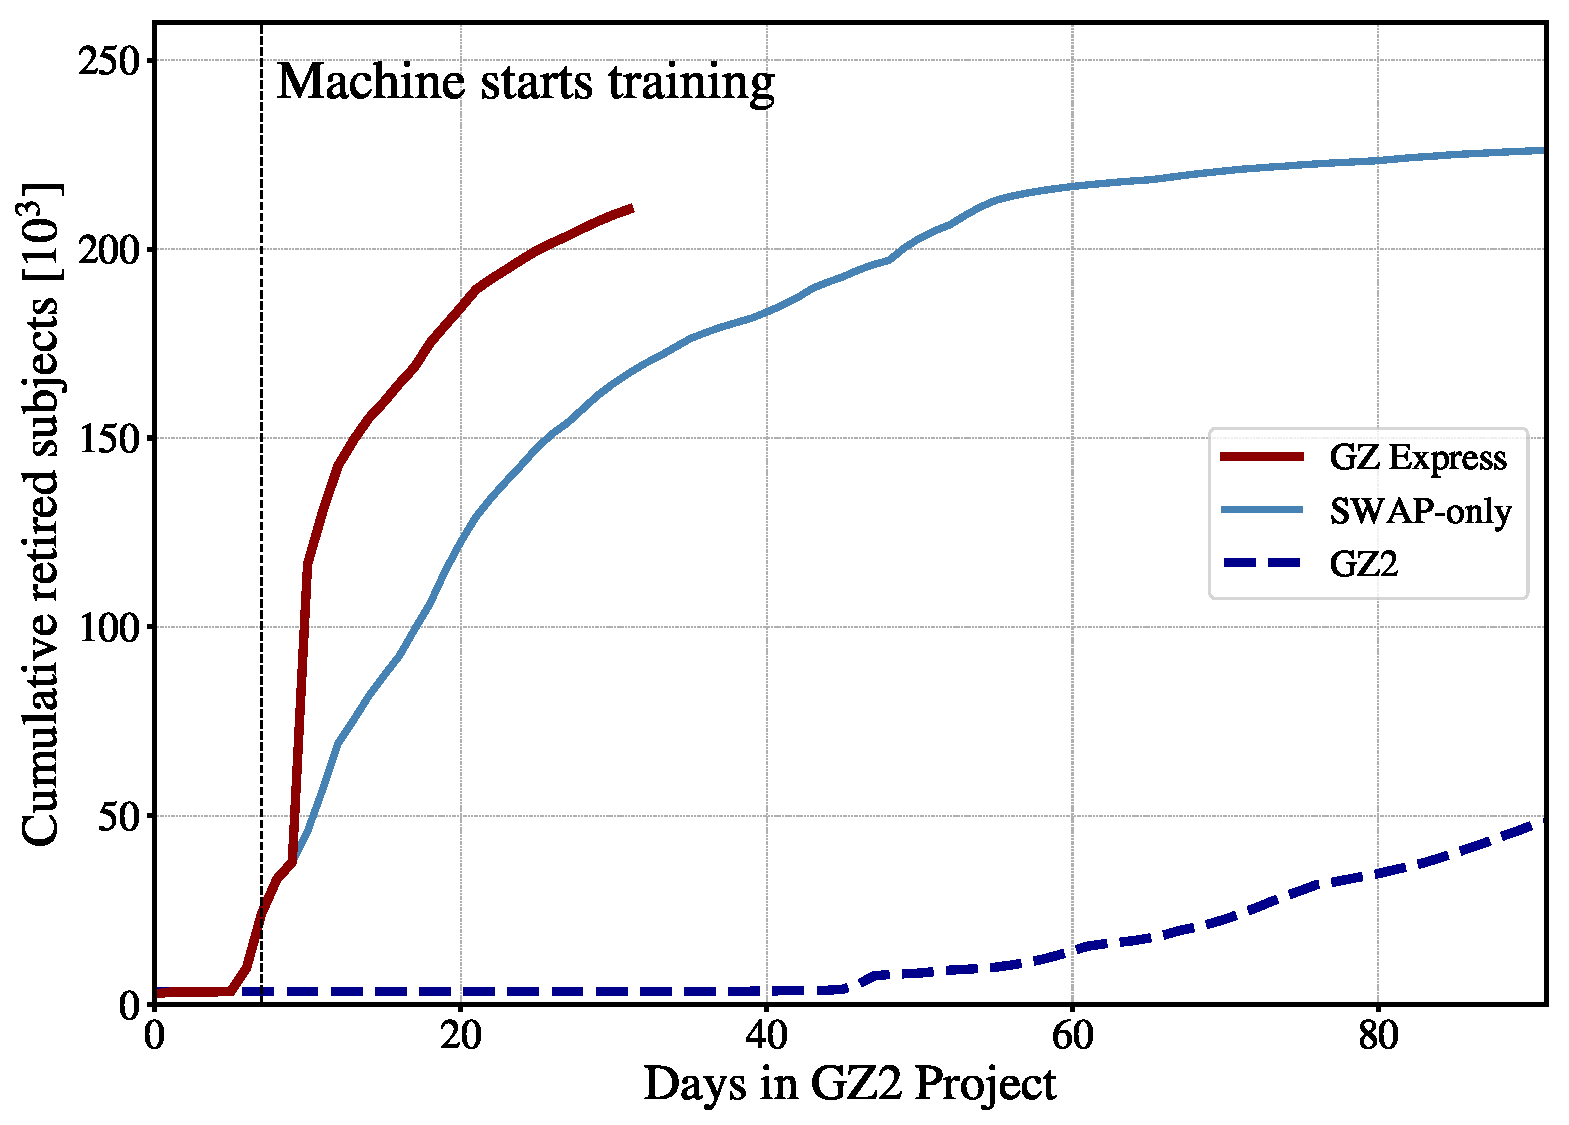
\includegraphics[width=7in]{Figures/human_machine/f10.pdf}
\caption[Distributions of measured galaxy morphology features.]{The RF is trained on a 5-dimensional morphology parameter space. We show the distribution of each morphology indicator for machine-retired~\feat~(blue) and~\notfeat~(orange) subjects compared to the full GZ2 subject sample (black). The difference between~\feat~and~\notfeat~subjects is in stark contrast for all distributions except, perhaps, \M{20}.  \label{fig: morph params}}
\end{figure*}

In the bottom panels of Figure~\ref{fig: gzx components}, we consider the class
composition of subjects retired by SWAP and the RF. 
The left (right) panel shows the retired fraction of GZ2 subjects identified 
as~\feat~(\notfeat) according to their~\raw~labels as a function of GZ2 project time. 
Overall, GZX retires 73.6\% of the GZ2 subject sample and this is evenly 
distributed between~\feat~and~\notfeat~subjects as indicated by the solid
black lines in both panels. 
However, SWAP retires more than 50\% of all~\feat~subjects while the machine
retires only 18\%. This divergence does not exist for~\notfeat~subjects where
each component contributes 33-37\%. 

What is the source of this discrepancy? 
Each night the machine trains on a sample composed consistently of 30-40\%~\feat~subjects but does not retire a similar proportion, indicating
that the 30\% of non-retired~\feat~subjects do not receive high~\pmachine. 
In the following section we explore whether this is an artefact of our choice in machine 
or in the human-machine combination implemented here. 

\subsection{Machine performance}\label{sec: machine performance}

Throughout our analysis we have defined~\feat~and~\notfeat~subjects by 
their~\raw~labels as this was the most compatible choice for comparison with SWAP output.  
However, the machine does not learn in the same way, nor is it presented with the 
same information. Machine and human classifications 
each provide valuable and complementary information for identifying \feat~galaxies.

We isolate the 6127 subjects that were deemed false positives, i.e., galaxies 
retired by the machine as~\feat~that have~\notfeat~\raw~labels, a sample that
comprises only 6.25\% of all subjects the machine retires.
We visually examine several hundred
and assess that, to the expert eye, a majority are, in fact, \feat.  
A random sample is shown in Figure~\ref{fig: machine false pos}. 


That the machine strongly identifies these galaxies as \feat~
(\pmachine~$\ge 0.9$) where humans instead classify them as \notfeat~(\ffeat~$< 0.5$) 
has several contributing factors: 1) as discussed in Section~\ref{sec: swap gz2 disagree}, 
the threshold we chose carries with it a confidence interval such that subjects with 
$0.4 <$~\ffeat+\fstar~$< 0.6$ are most likely to receive disagreeing labels from 
other classifying agents, 2) the first task of the GZ2 decision tree asks a 
question that does not necessarily correlate with a split between early- and
 late-type galaxies, and 3) the machine learns on morphology diagnostics
 that are very different from visual inspection.

We find that 41.4\% of these false positives have $0.4 \le$~\ffeat+\fstar$<0.5$ 
indicating that the disagreement between humans and machine is likely due to the 
labels we assign at our given threshold. However, we also find that 43.5\% of false 
positives have \ffeat+\fstar~$\le0.35$, and this discrepancy is not as easily explained. 
 In Figure~\ref{fig: machine false pos} we examine a random sample of false positives 
in this regime where, for clarity, we display only the \ffeat~value in the lower left corner. 
The majority of these subjects are discs lacking features such as spiral arms or strong bars. 
Whether this is the reason the majority of volunteers classify these objects as 
``smooth" is beyond the scope of this paper, however, this behaviour might be 
modified by providing actual training images and live feedback as performed in
 \cite{Marshall2016}. We suggest that, at least for this particular question, 
if either human or machine identifies a subject as \feat, it is likely the subject 
is discy and worth further investigation.


%%%-------------------------------------------------------
%%%  FIGURE:   FEATURE IMPORTANCES
%%%-------------------------------------------------------
\begin{figure}[t]
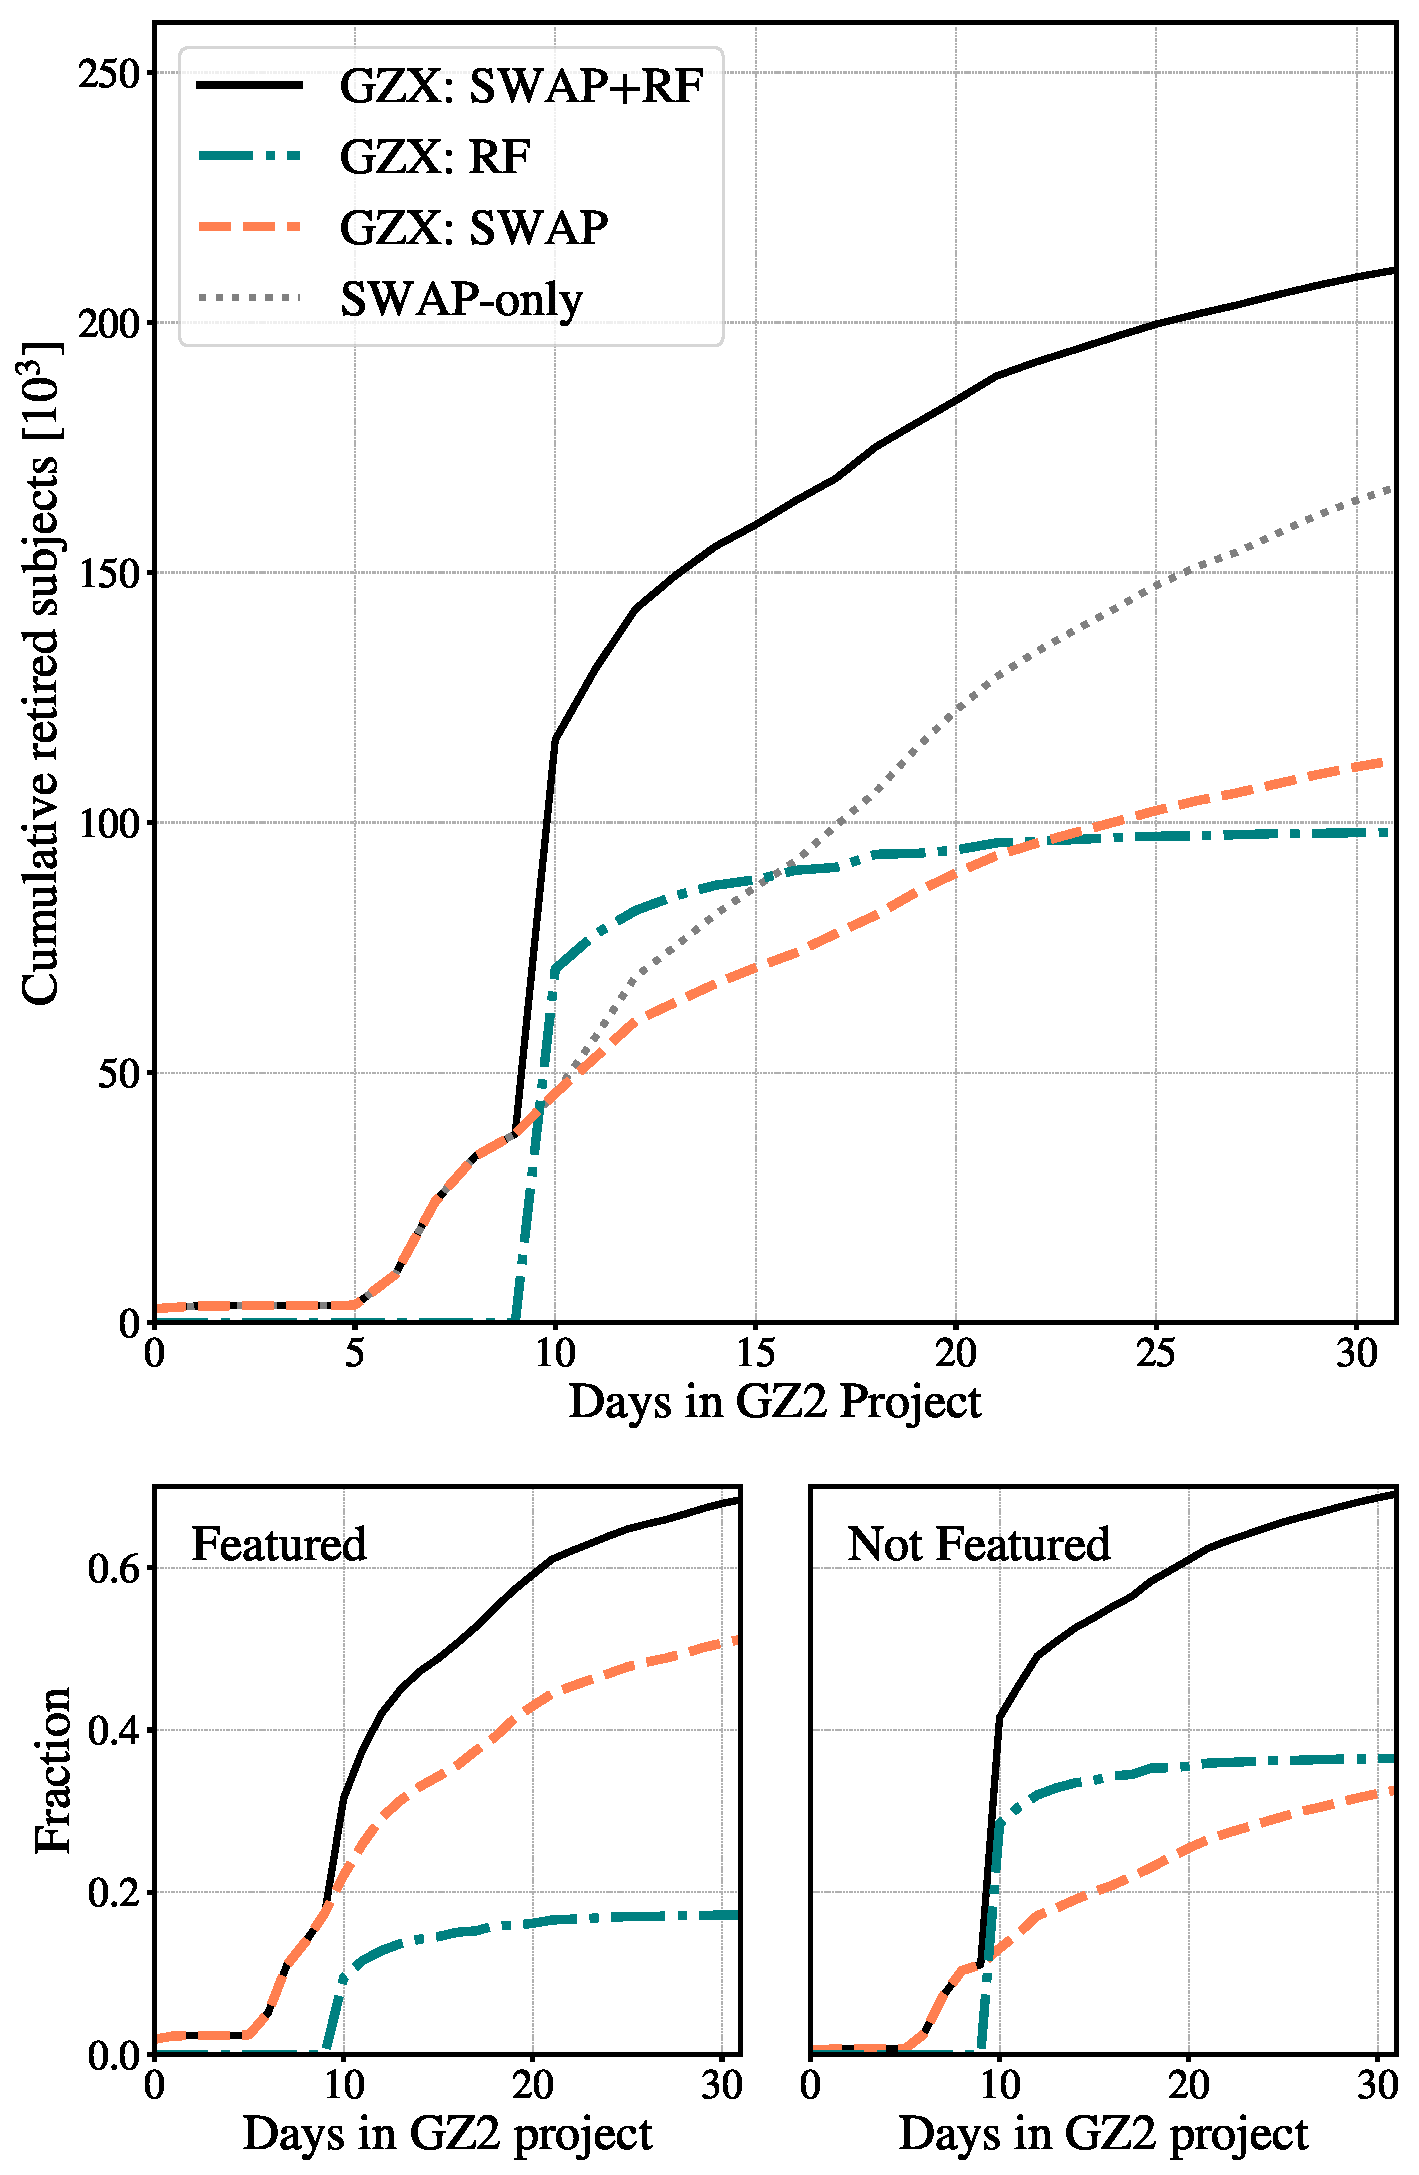
\includegraphics[width=3.5in]{Figures/human_machine/f11.pdf}
\caption[Random Forest's feature importances]{The RF's ranked feature importance averaged over all nights of training with black bars indicating the standard deviation. A larger value corresponds to higher importance. The machine computes feature importance according to how much each feature increases the purity of the resulting split averaged over all trees in the forest. The RF places great importance in the Gini coefficient though we note that it can under-represent the importance of highly correlated features such as concentration.\label{fig: feature importance}}
\end{figure}

Accordingly, this suggests that, in some cases, the morphology indicators we measure are 
sufficient for the machine to recognize~\feat~galaxies regardless of the labels humans provide. 
Figure~\ref{fig: morph params} shows the distribution of each 
morphology indicator for all subjects the machine retires as~\feat~(blue) 
and~\notfeat~(orange) compared to the full GZ2 subject set. 
The difference between~\feat~and~\notfeat~is stark in all but the \M{20} distribution. 
This can be seen explicitly in Figure~\ref{fig:  feature importance} in which
we show the RF's ranked feature importances, where large values indicate higher importance. 
Feature importance is computed as how much each feature decreases the impurity 
of a split in a tree. The impurity decrease from each feature is then averaged over
all trees and ranked. 
We show the feature importance averaged over all nights of training with 
black bars indicating the standard deviation. The machine finds the Gini coefficient 
most important for class prediction, placing little emphasis on \M{20}. 
It is well known that the Gini coefficient is more sensitive to noise than other diagnostics, 
however, we point out that when a machine is faced with two or more correlated features 
any of them can be used as the predictor. Once chosen, the importance of the others is reduced. 
This explains why Concentration is ranked much lower than Gini even though they 
are strongly correlated as seen in Figure~\ref{fig: morph thresh}. 
That the machine relies heavily on these two morphology diagnostics is unsurprising as
concentration has long been an automated predictor between early- and late-type galaxies~\citep{Abraham1994, Abraham1996, Shen2003}.


The complementary nature of human and machine classification can 
best be utilized by a feedback mechanism in which a portion of machine-retired
subjects are reviewed by humans. Subjects that display excessive disagreement
should be verified by an expert (or expert-user).  In the same way that 
humans increase the machine's training sample over time, subjects that the
machine properly identifies can become part of the humans' training sample. 



%%----------------------------------------------------------------------------------------------------------------------------------------------------
%%   MAD RAVINGS OF THE FUTURE 
%%----------------------------------------------------------------------------------------------------------------------------------------------------
\section{Looking Forward}\label{sec: visions}

We have demonstrated the first practical framework for combining human and machine
 intelligence in galaxy morphology classification tasks. 
While we focus below on a brief discussion of our next steps and potential applications
to large upcoming surveys, we note that our results have implications for the future
of citizen science and Galaxy Zoo in particular. 


GZX is perhaps one of the simplest ways to combine human and machine intelligence
 and its impressive performance motivates a higher level of sophistication. 
A first step will be an implementation of SWAP that can handle a complex decision tree. 
In addition, we envision multiple forms of active feedback in addition to 
our passive feedback mechanism.  SWAP allows us to leverage the 
most skilled volunteers to review galaxies difficult for either
 human or machine to classify.  Additionally, machine-retired subjects should 
contribute to the training sample for humans in an analogous fashion to what 
we have already implemented. 


Secondly, our RF can be improved by providing it information equal to what
humans receive: multi-band morphology diagnostics will be
included in our future feature vector.  However, the Random Forest algorithm is not 
easily adapted to handle measurement errors or class labels with continuous distributions. 
To fully utilize the information provided by SWAP, sophisticated algorithms should be considered such as 
deep convolutional neural networks (CNN) or Latent Dirichlet allocation (LDA), 
an algorithm that is frequently used in document processing.  
Furthermore, there is no reason to limit to a single machine. 
As hinted at in Figure~\ref{fig: schematic}, several machines could train simultaneously, 
their predictions aggregated through SWAP, creating an on-the-fly machine ensemble.

%%----------------------------------------------------------------------------------------------------------------------------------------------------
%%  IMPLICATIONS FOR UPCOMING LARGE-SCALE SURVEYS
%%----------------------------------------------------------------------------------------------------------------------------------------------------

With the above upgrades implemented, we expect performance of both the
classification rate and quality to further increase. However, even our current 
implementation can cope with upcoming data volumes from large surveys. 
By some estimates, \textit{Euclid} is expected to obtain measurable morphology with its 
visual instrument (VIS) for approximately $10^6 - 10^7$ galaxies~\citep{Euclid}.
Visual classification at the rate achieved with Galaxy Zoo today
would require 12--120 years to classify.\footnote{We note that the classification 
rate of GZ2 was 4 times higher than GZ's current steady rate.}
If the \textit{Euclid} sample is on the high end, GZX as currently implemented
could classify the brightest 20\% during the six years of its observing mission. 
As currently implemented, we obtain accuracy around 95\% potentially leaving
hundreds of thousands of galaxies with unreliable classifications.  
In a companion paper that seeks to identify supernovae, Wright et al. (submitted) 
demonstrate a dramatic increase in accuracy through an entirely different human-machine 
combination whereby the
scores from human and machine are averaged together with the combined score 
yielding the most reliable classification. Again, a combination of both 
approaches will allow us to take full advantage of legacy output from large scale surveys.


%%----------------------------------------------------------------------------------------------------------------------------------------------------
%%   CONCLUSIONS 
%%----------------------------------------------------------------------------------------------------------------------------------------------------
\subsection{Conclusions}

In this paper we design and test Galaxy Zoo Express, an innovative system\footnote{Our code can be found at \url{https://github.com/melaniebeck/GZExpress}} 
for the efficient classification of galaxy morphology tasks that integrates the 
native ability of the human mind to identify the abstract and novel with 
machine learning algorithms that provide speed and brute force.  
We demonstrate for the first time that the 
SWAP algorithm, originally developed to identify rare gravitational lenses in the 
Space Warps project, is robust for use in galaxy morphology classification. 
We show that by implementing
SWAP on GZ2 classification data we can increase the rate of classification by a factor
of 4-5, requiring only 90 days of GZ2 project time to classify nearly 80\% of the
entire galaxy sample. 

Furthermore, we have implemented and tested a Random Forest algorithm 
and developed a decision engine that delegates tasks between human and 
machine.  We show that even this simple machine is capable of providing significant 
gains in the classification rate when combined with human classifiers: GZX
 retires over 70\% of GZ2 galaxies in just 32 days of GZ2 project time.  
This represents a factor of 11.4 increase in the classification rate as well as
 an order of magnitude reduction in human effort compared to the original GZ2 project. 
This is achieved without sacrificing the quality of classifications as we maintain 
accuracy well above 90\% throughout our simulations. 
Additionally, we have shown that training on a 5-dimensional parameter space of 
traditional non-parametric morphology indicators allows the machine to identify 
subjects that humans miss, providing  a complementary approach to visual classification. 
The gain in classification speed allows us to tackle the massive amount of data promised
 from large surveys like \textit{LSST} and \textit{Euclid}.
 
 
%%----------------------------------------------------------------------------------------------------------------------------------------------------
%%   ACKNOWLEDGEMENTS
%%----------------------------------------------------------------------------------------------------------------------------------------------------
\section{Acknowledgements}
MB thanks Steven Bamford and Boris H{\"a}u{\ss}ler for insightful discussions on citizen science and Galaxy Zoo; and John Wallin and Marc Huertas-Company for several enlightening conversations on machine learning and classification. 
We are grateful to Elisabeth Baeten, Micaela Bagley, Karlen Shahinyan, Vihang Mehta, Steven Bamford, Kevin Schawinski, and Rebecca Smethurst for providing expert classifications in addition to those provided by the authors. PJM acknowledges Aprajita Verma and Anupreeta More for their ongoing collaboration on the Space Warps project. 

MB, CS, LF, KW, and MG gratefully acknowledge support from the US National Science
Foundation Grant AST-1413610.  MB acknowledges additional support 
through New College and Oxford University's Balzan Fellowship as well as the University
of Minnesota Doctoral Dissertation Fellowship. Travel funding was supplied 
to MB, in part, by the University of Minnesota Thesis Research Travel Grant. CJL recognizes support from a grant from the Science \& Technology Facilities Council (ST/N003179/1). 
BDS acknowledges support from Balliol College, Oxford, and the National Aeronautics and Space Administration (NASA) through Einstein Postdoctoral Fellowship Award Number PF5-160143 issued by the Chandra X-ray Observatory Center, which is operated by the Smithsonian Astrophysical Observatory for and on behalf of NASA under contract NAS8-03060. The work of PJM is supported by the U.S. Department of Energy under contract number DE-AC02-76SF00515.
